In this section,
the performance of the proposed method is evaluated in comparison with baselines.
To support the evaluation,
different simulated tasks with varying difficulty levels ranging from simple to complex ones were utilized.
The details of these tasks are described in the next subsection.
A set of experiments are designed in order to answer the following essential questions:


\begin{itemize}
  \item Can the proposed IL agent provide a competitive performance on the source task?
  \item Can the adaptation algorithm enable the agent to adapt its learned knowledge to the target task in order to outperform the baselines?
  \item By leveraging the repetition learning to expand the agent's knowledge, can the adaptation algorithm reduce the deterioration of the agent's performance on the source task?
\end{itemize}


\subsection{Experimental Settings}
\subsubsection{Simulated Tasks}


In order to examine the effectiveness of the proposed method,
six simulated tasks with varying difficulties were considered:
Pendulum \cite{Env_OpenAIGym},
CartPole \cite{Env_OpenAIGym, Env_CartPole},
WindowOpen \cite{Env_MetaWorld},
WindowClose \cite{Env_MetaWorld},
Door \cite{Env_Adroit},
and Hammer \cite{Env_Adroit}.
The task difficulty is varied along two axes;
the size of the state space and the size of the action space.
The detailed descriptions and visualizations of these tasks are shown in Table \ref{ch:DTAIL:tab:Tasks} and Figure \ref{ch:DTAIL:fig:Tasks}.
From such tasks,
three experiments were conducted,
each of which included two different tasks---a source task and a target task.
The detailed descriptions of these experiments are shown in Table \ref{ch:DTAIL:tab:Experiments}.

\begin{landscape}
  \begin{table}[htbp!]
    \caption{Description of six simulated tasks used in the experiment.\label{ch:DTAIL:tab:Tasks}}

    \begin{tabular}{lcccp{5.5cm}}
      \toprule
      \textbf{Task}                               & \textbf{Size of State Space} & \textbf{Size of Action Space}                                              & \textbf{Difficulty Level} & \textbf{Description} \\
      \midrule
      Pendulum \cite{Env_OpenAIGym}               & 3 (continuous)               & 1 (continuous)
                                                  & Easy                         & Swinging up a pendulum.                                                                                                       \\
      CartPole \cite{Env_OpenAIGym, Env_CartPole} & 4 (continuous)               & 1 (continuous)
                                                  & Easy                         & Preventing the pendulum from falling over by applying a force to the cart.                                                    \\
      WindowOpen \cite{Env_MetaWorld}             & 39 (continuous)              & 4 (continuous)
                                                  & Medium                       & Opening a window.                                                                                                             \\
      WindowClose \cite{Env_MetaWorld}            & 39 (continuous)              & 4 (continuous)
                                                  & Medium                       & Closing a window.                                                                                                             \\
      Door \cite{Env_Adroit}                      & 39 (continuous)              & 28 (continuous)
                                                  & Hard                         & A 24-DoF hand attempts to undo the latch and swing the door open.                                                             \\
      Hammer \cite{Env_Adroit}                    & 46 (continuous)              & 26 (continuous)
                                                  & Hard                         & A 24-DoF hand attempts to use a hammer to drive the nail into the board.                                                      \\
      \bottomrule
    \end{tabular}
  \end{table}

  \begin{table}[H]
    \centering
    \caption{Description of three experiments conducted to evaluate the performance of the proposed method.\label{ch:DTAIL:tab:Experiments}}

    \begin{tabular}{lcccp{5.5cm}}
      \toprule
      \textbf{Experiment}     & \textbf{Source Task} & \textbf{Target Task}                                                                               & \textbf{Difficulty Level} & \textbf{Description} \\
      \midrule
      Pendulum--CartPole      & Pendulum             & CartPole
                              & Easy                 & A simple experiment in which both source and target tasks have small state and action spaces.                                                         \\
      WindowOpen--WindowClose & WindowOpen           & WindowClose
                              & Medium               & Both source and target tasks have a large state space but small action space.                                                                         \\
      Door--Hammer            & Door                 & Human
                              & Hard                 & A challenging experiment in which both source and target tasks have large state and action spaces.                                                    \\
      \bottomrule
    \end{tabular}
  \end{table}
\end{landscape}

\begin{figure}[H]
  \centering
  \begin{subfigure}[b]{0.2\textwidth}
    \centering
    \frame{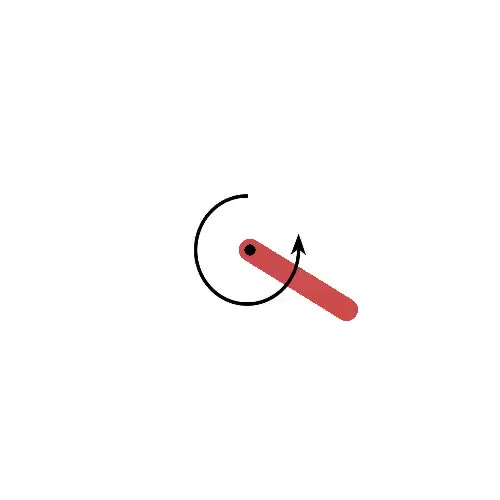
\includegraphics[width=\textwidth]{\FigsDir/Pendulum.jpg}}
    \caption{Pendulum}
  \end{subfigure}
  %
  \hfill
  %
  \begin{subfigure}[b]{0.2\textwidth}
    \centering
    \frame{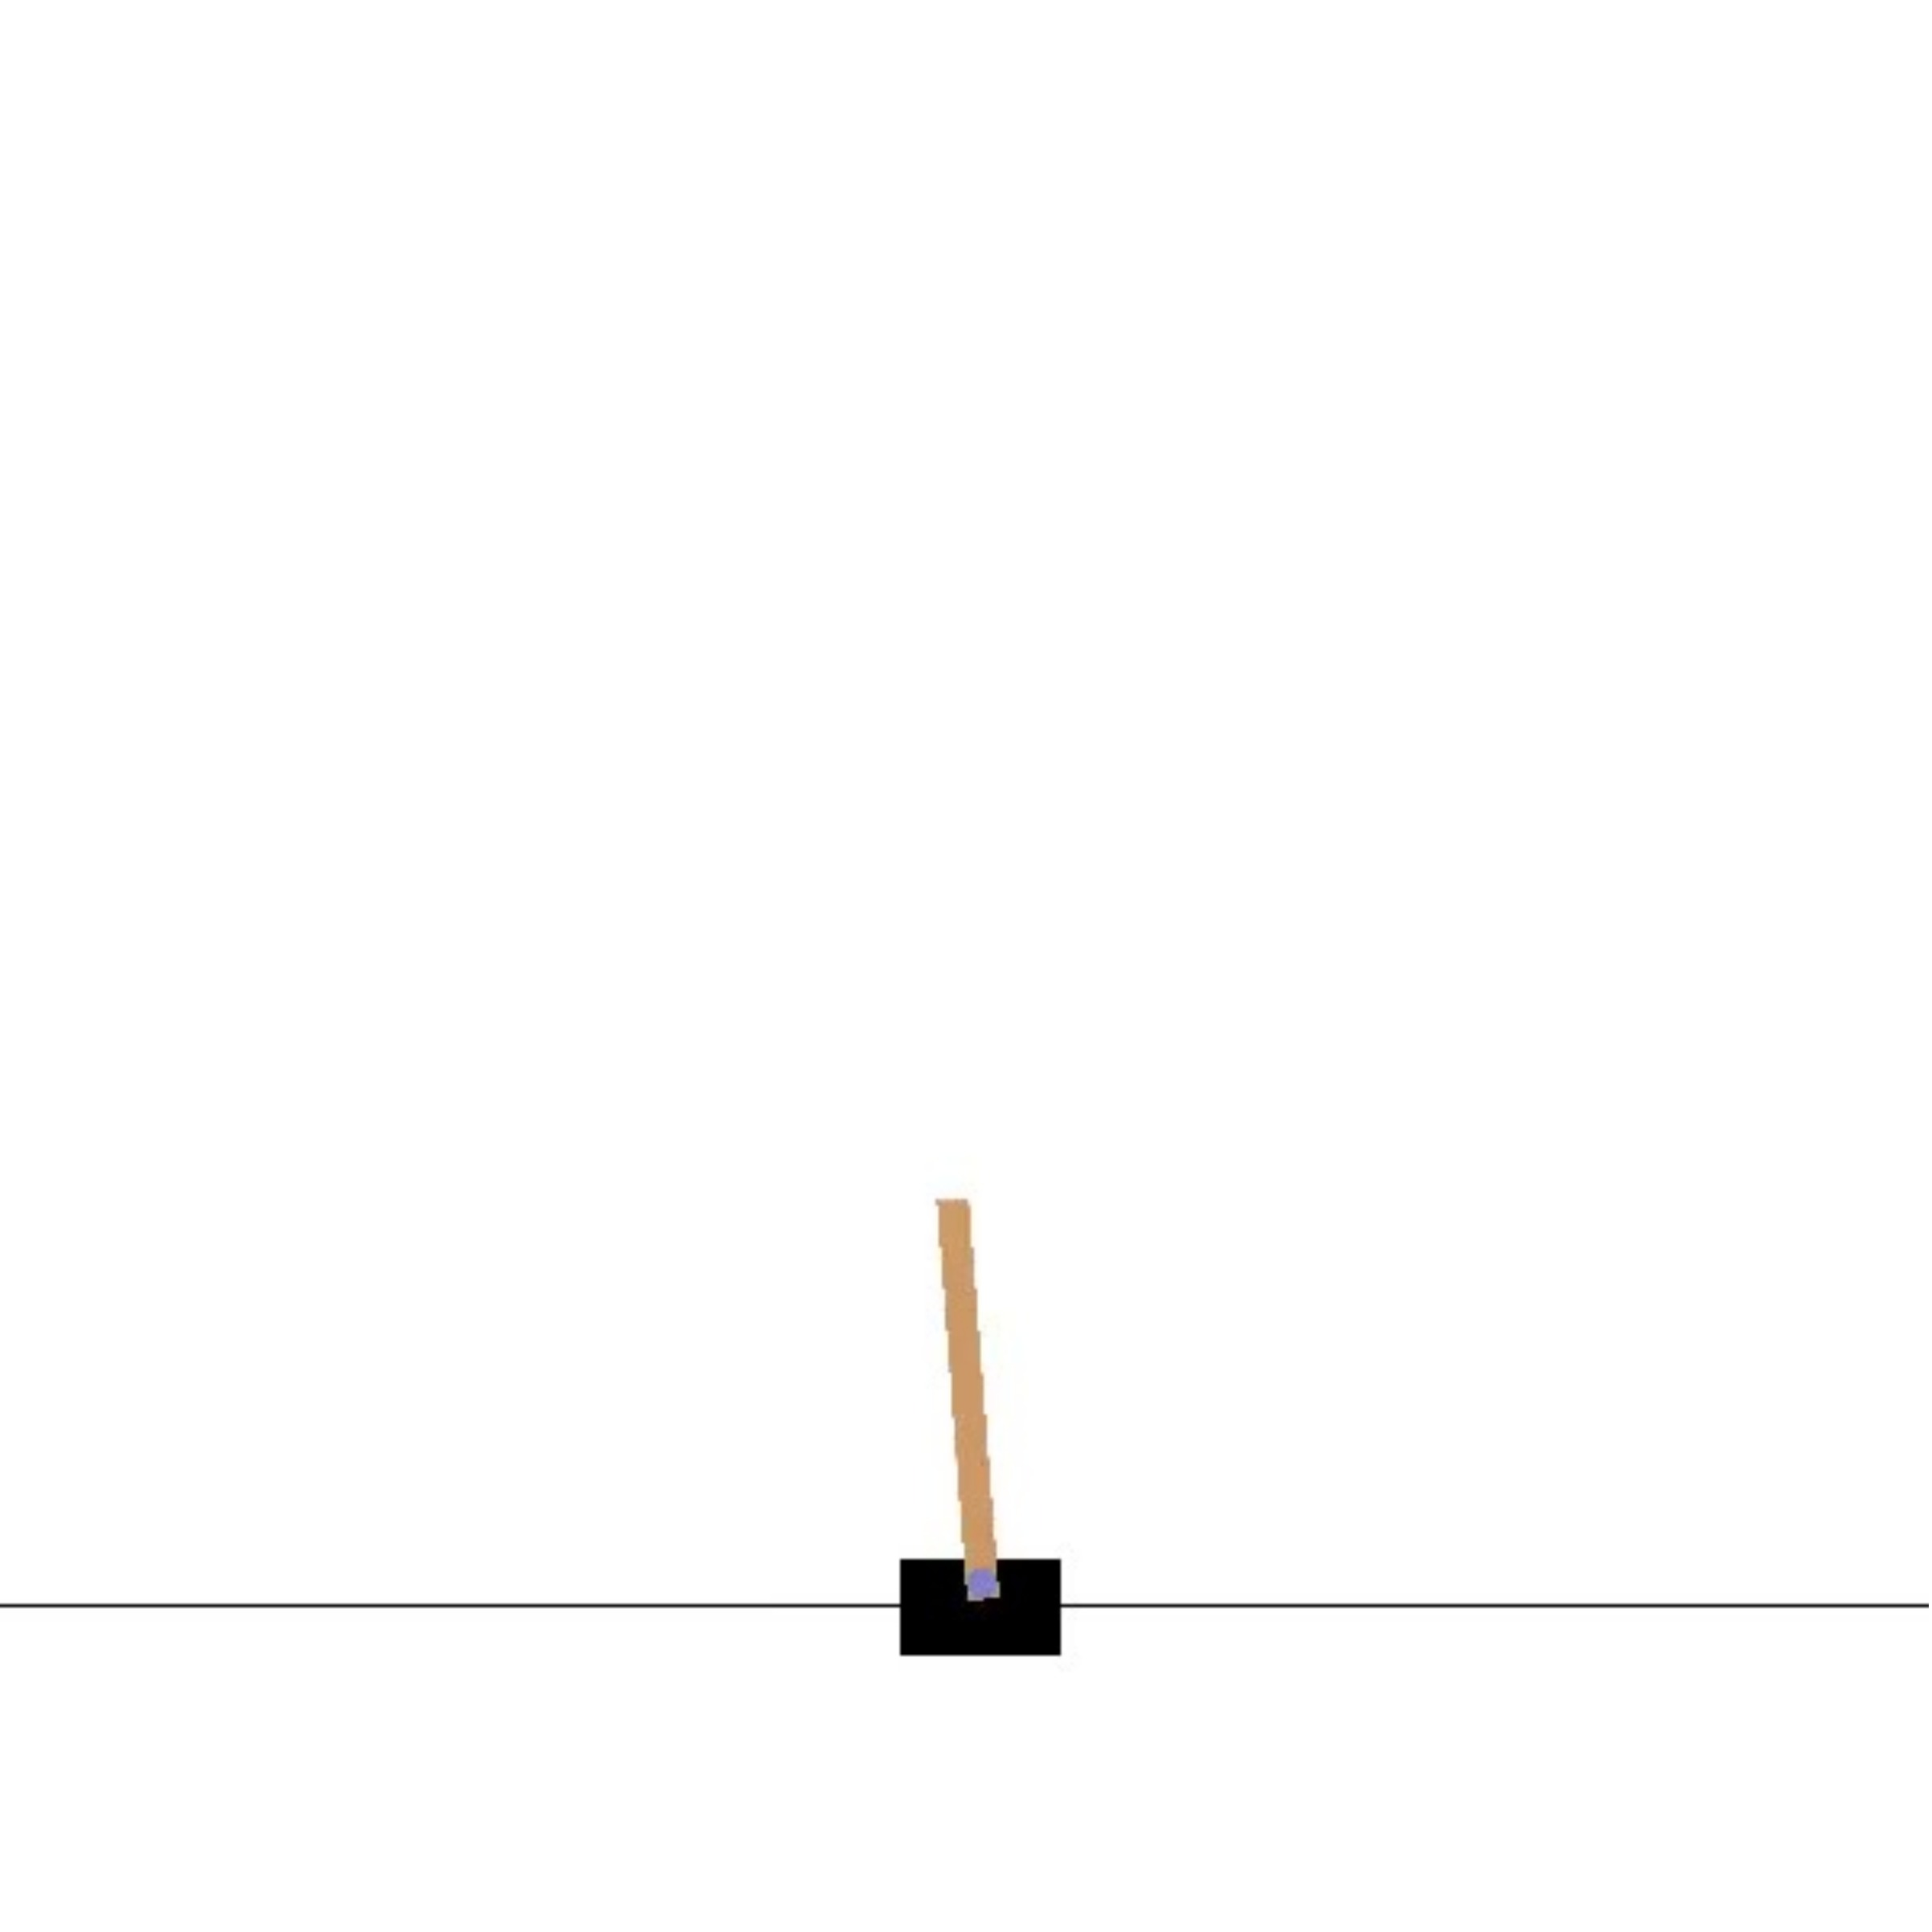
\includegraphics[width=\textwidth]{\FigsDir/CartPole.jpg}}
    \caption{CartPole}
  \end{subfigure}
  %
  \hfill
  %
  \begin{subfigure}[b]{0.25\textwidth}
    \centering
    \frame{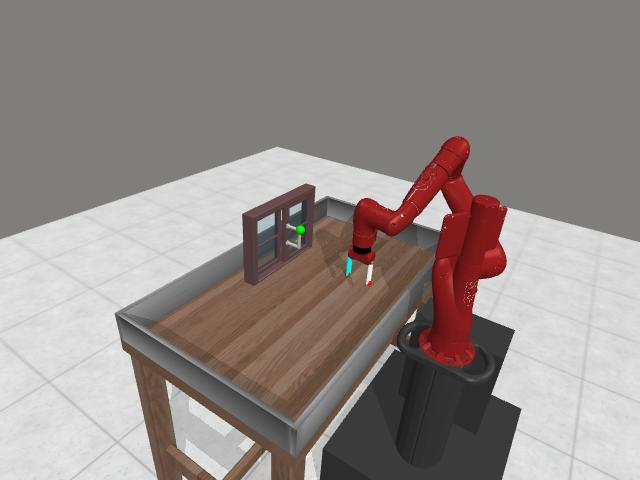
\includegraphics[width=\textwidth]{\FigsDir/WindowOpen.jpg}}
    \caption{WindowOpen}
  \end{subfigure}
  %
  \hfill
  %
  \begin{subfigure}[b]{0.25\textwidth}
    \centering
    \frame{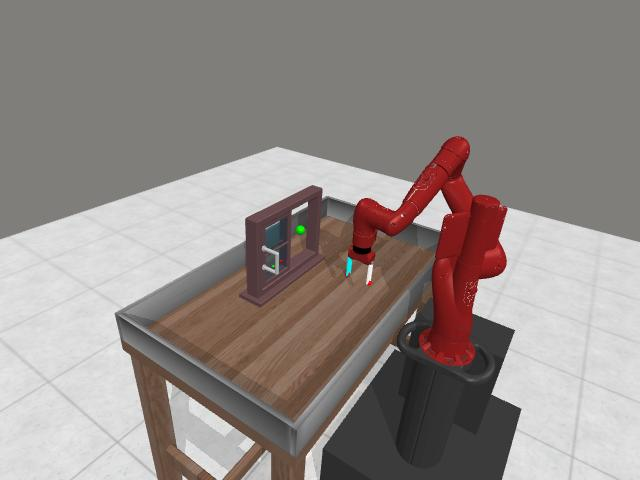
\includegraphics[width=\linewidth]{\FigsDir/WindowClose.jpg}}
    \caption{WindowClose}
  \end{subfigure}\\
  %
  \par\bigskip
  %
  \begin{subfigure}[b]{0.2\textwidth}
    \centering
    \frame{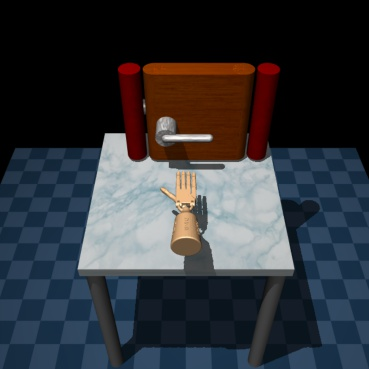
\includegraphics[width=\linewidth]{\FigsDir/Door.jpg}}
    \caption{Door}
  \end{subfigure}
  %
  % \hfill
  %
  \hspace{4em}
  \begin{subfigure}[b]{0.2\textwidth}
    \centering
    \frame{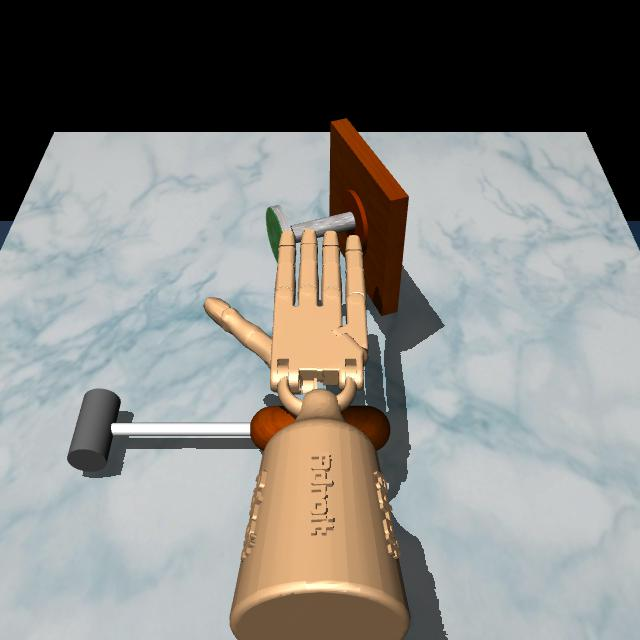
\includegraphics[width=\linewidth]{\FigsDir/Hammer.jpg}}
    \caption{Hammer}
  \end{subfigure}
  %
  \caption{Visual rendering of five simulated tasks used in the experiment.\label{ch:DTAIL:fig:Tasks}}
\end{figure}
\unskip




In order to train and adapt the proposed IL agent,
expert demonstrations for both source and target tasks must be provided.
In this experiment,
the proximal policy optimization (PPO) method was chosen to be trained on each task in order to create an expert RL agent.
The reason behind this decision was that PPO was recently showing the best result for many complex tasks.
After that,
the demonstrations were collected by executing the trained PPO expert agent in the simulated task under different configurations.
For the source task, 30 demonstrations were collected to provide sufficient data for training the proposed agent \cite{IL_Model_GAIL}.
In the adaptation process, the proposed agent already learned the knowledge of the source task, thus, a smaller number of demonstrations for the target task is required.
Therefore, only 15 demonstrations were collected for the target task.


%==================================================
\subsubsection{Baselines}


To evaluate the performance of the proposed method,
a number of baselines were considered.
Firstly,
to assess the performance of the proposed agent on a source task,
two RL baselines were used, which are proximal policy optimization (PPO) \cite{Baseline_PPO} and neural fitted Q-iteration (NFQI) \cite{Baseline_NFQI}.
PPO is a policy gradient method,
while NFQI is a value-based method that tries to estimate the Q-function using a deep feed-forward network.
Secondly,
after training the agent on the source task,
the proposed adaptation algorithm was applied in order to adapt the trained agent to a new target task.
The performance of the agent after adaptation was evaluated through the comparison with transfer learning-based baselines, which are fine-tuning and TA-TL \cite{Baseline_TATL}.
Fine-tuning is a common transfer learning technique that simply re-trains the agent on a new target task.
Fine-tuning was applied to both the proposed agent and PPO,
resulting in two baselines for the evaluation.
Meanwhile,
TA-TL is a policy adaptation method, where first it utilizes the NFQI agent to find an optimal policy on a source task,
then that policy is transferred to a new target task.
In order to provide a fair comparison,
each baseline was evaluated for 100 trials.
The success rate and average cumulative reward were used as performance metrics.
The success rate indicates the percentage of trials in which the baseline can successfully complete a task.
The average cumulative reward measures how well the baseline performed in a trial.


%==================================================
\subsubsection{Implementation and Training Details}


In order to perform the experiments,
a personal computer running Ubuntu 20.04 with an Intel i7-8750H @ 2.20GHz,
16 GB RAM,
and NVIDIA GTX 1080 Ti was used.
PyTorch \cite{DL_Lib_PyTorch} and Tianshou \cite{DL_Lib_Tianshou} were utilized as deep learning frameworks to implement the proposed adaptation method and baselines.
Adam optimizer with an initial learning rate of $10^{-4}$ was used for training the proposed agent.
The dimension $n$ of the task embedding $z^t_x$ and the value of $\lambda$ were set to $64$ and $0.1$, respectively.


\subsection{Results}
In this subsection, the evaluation results of the proposed agent and adaptation algorithm are presented to highlight their effectiveness in tackling the domain and task adaptation problem in imitation learning.

\subsubsection{Performance of the Proposed Agent on the Source Task}
Table \ref{ch:DTAIL:tab:Result_SuccessRate_Before_Source} reports the performance of the proposed agent on the source tasks (i.e., Pendulum, WindowOpen, and Door) against two RL baselines: PPO and NFQI.
In addition,
Figure \ref{ch:DTAIL:fig:Result_Before_Source} visualizes their behaviors when performing the source tasks.
It can be observed that the proposed agent and two baselines could accomplish source tasks by keeping the pendulum vertical (Figure \ref{ch:DTAIL:fig:Result_Before_Source}a), successfully opening the window and the door (\mbox{Figure \ref{ch:DTAIL:fig:Result_Before_Source}b,c)}.
The proposed imitation learning agent was able to produce relatively similar behaviors to PPO.
This result demonstrated that the proposed agent was trained successfully in order to imitate the expert behaviors.
Table \ref{ch:DTAIL:tab:Result_SuccessRate_Before_Source} shows that PPO always provided the best performance in terms of success rate
and average cumulative reward
on three different source tasks.
This result was reasonable since PPO is a reinforcement learning method,
thus,
it has a direct access to the task environment, including states and the reward signal.
On the other hand,
the proposed agent is an imitation learning method that learns to perform the task using only expert demonstrations.
Despite that disadvantage,
the proposed agent could consistently perform well on all source tasks with varying difficulties and almost achieved similarly high performance to PPO.
It should be noted that the performance of all agents always decreased when being tested on a more complicated task with more extensive state and action spaces,
especially the Door task.
However, the reduction in performance between the proposed agent and PPO was comparable.
On the other hand,
there was a significant gap between the proposed agent and the NFQI performance.
The NFQI agent showed the largest reduction in terms of success rate,
i.e., from 100\% success rate on the simple Pendulum task to only 65\% on the challenging Door task.
This was because the Q-function approximation in NFQI did not work well with the task with large state and action spaces \cite{Baseline_NFQI}.
In summary, the results showed that the proposed agent could provide relatively high and consistent performance that is close to the expert PPO on different source tasks with various difficulty levels.


\begin{landscape}
  \begin{table}[H]
    \caption{The performance of the proposed agent on source tasks.} \label{ch:DTAIL:tab:Result_SuccessRate_Before_Source}

    %\centering
    \begin{tabular}{llccc}
      \toprule
                                    &                           & \textbf{Pendulum}     & \textbf{WindowOpen}  & \textbf{Door}         \\
      \midrule
      \multirow{3}{*}{Success rate} & \DTAIL{}                  & 100\%                 & 94\%                 & 87\%                  \\
                                    & PPO \cite{Baseline_PPO}   & 100\%                 & 97\%                 & 91\%                  \\
                                    & NFQI \cite{Baseline_NFQI} & 100\%                 & 76\%                 & 65\%                  \\
      \midrule
      \multirow{3}{*}{Average cumulative reward}
                                    & \DTAIL{}                  & $-$146.51 $\pm$ 85.24 & 1586.38 $\pm$ 229.00 & 2250.04 $\pm$ 1428.60 \\
                                    & PPO \cite{Baseline_PPO}   & $-$134.77 $\pm$ 93.59 & 1827.56 $\pm$ 410.98 & 2450.42 $\pm$ 1303.48 \\
                                    & NFQI \cite{Baseline_NFQI} & $-$189.01 $\pm$ 87.09 & 752.00 $\pm$ 476.77  & 1252.55 $\pm$ 1213.15 \\
      \bottomrule
    \end{tabular}
  \end{table}







  \begin{figure}[H]
    \centering
    \begin{subfigure}[b]{\linewidth}
      \centering
      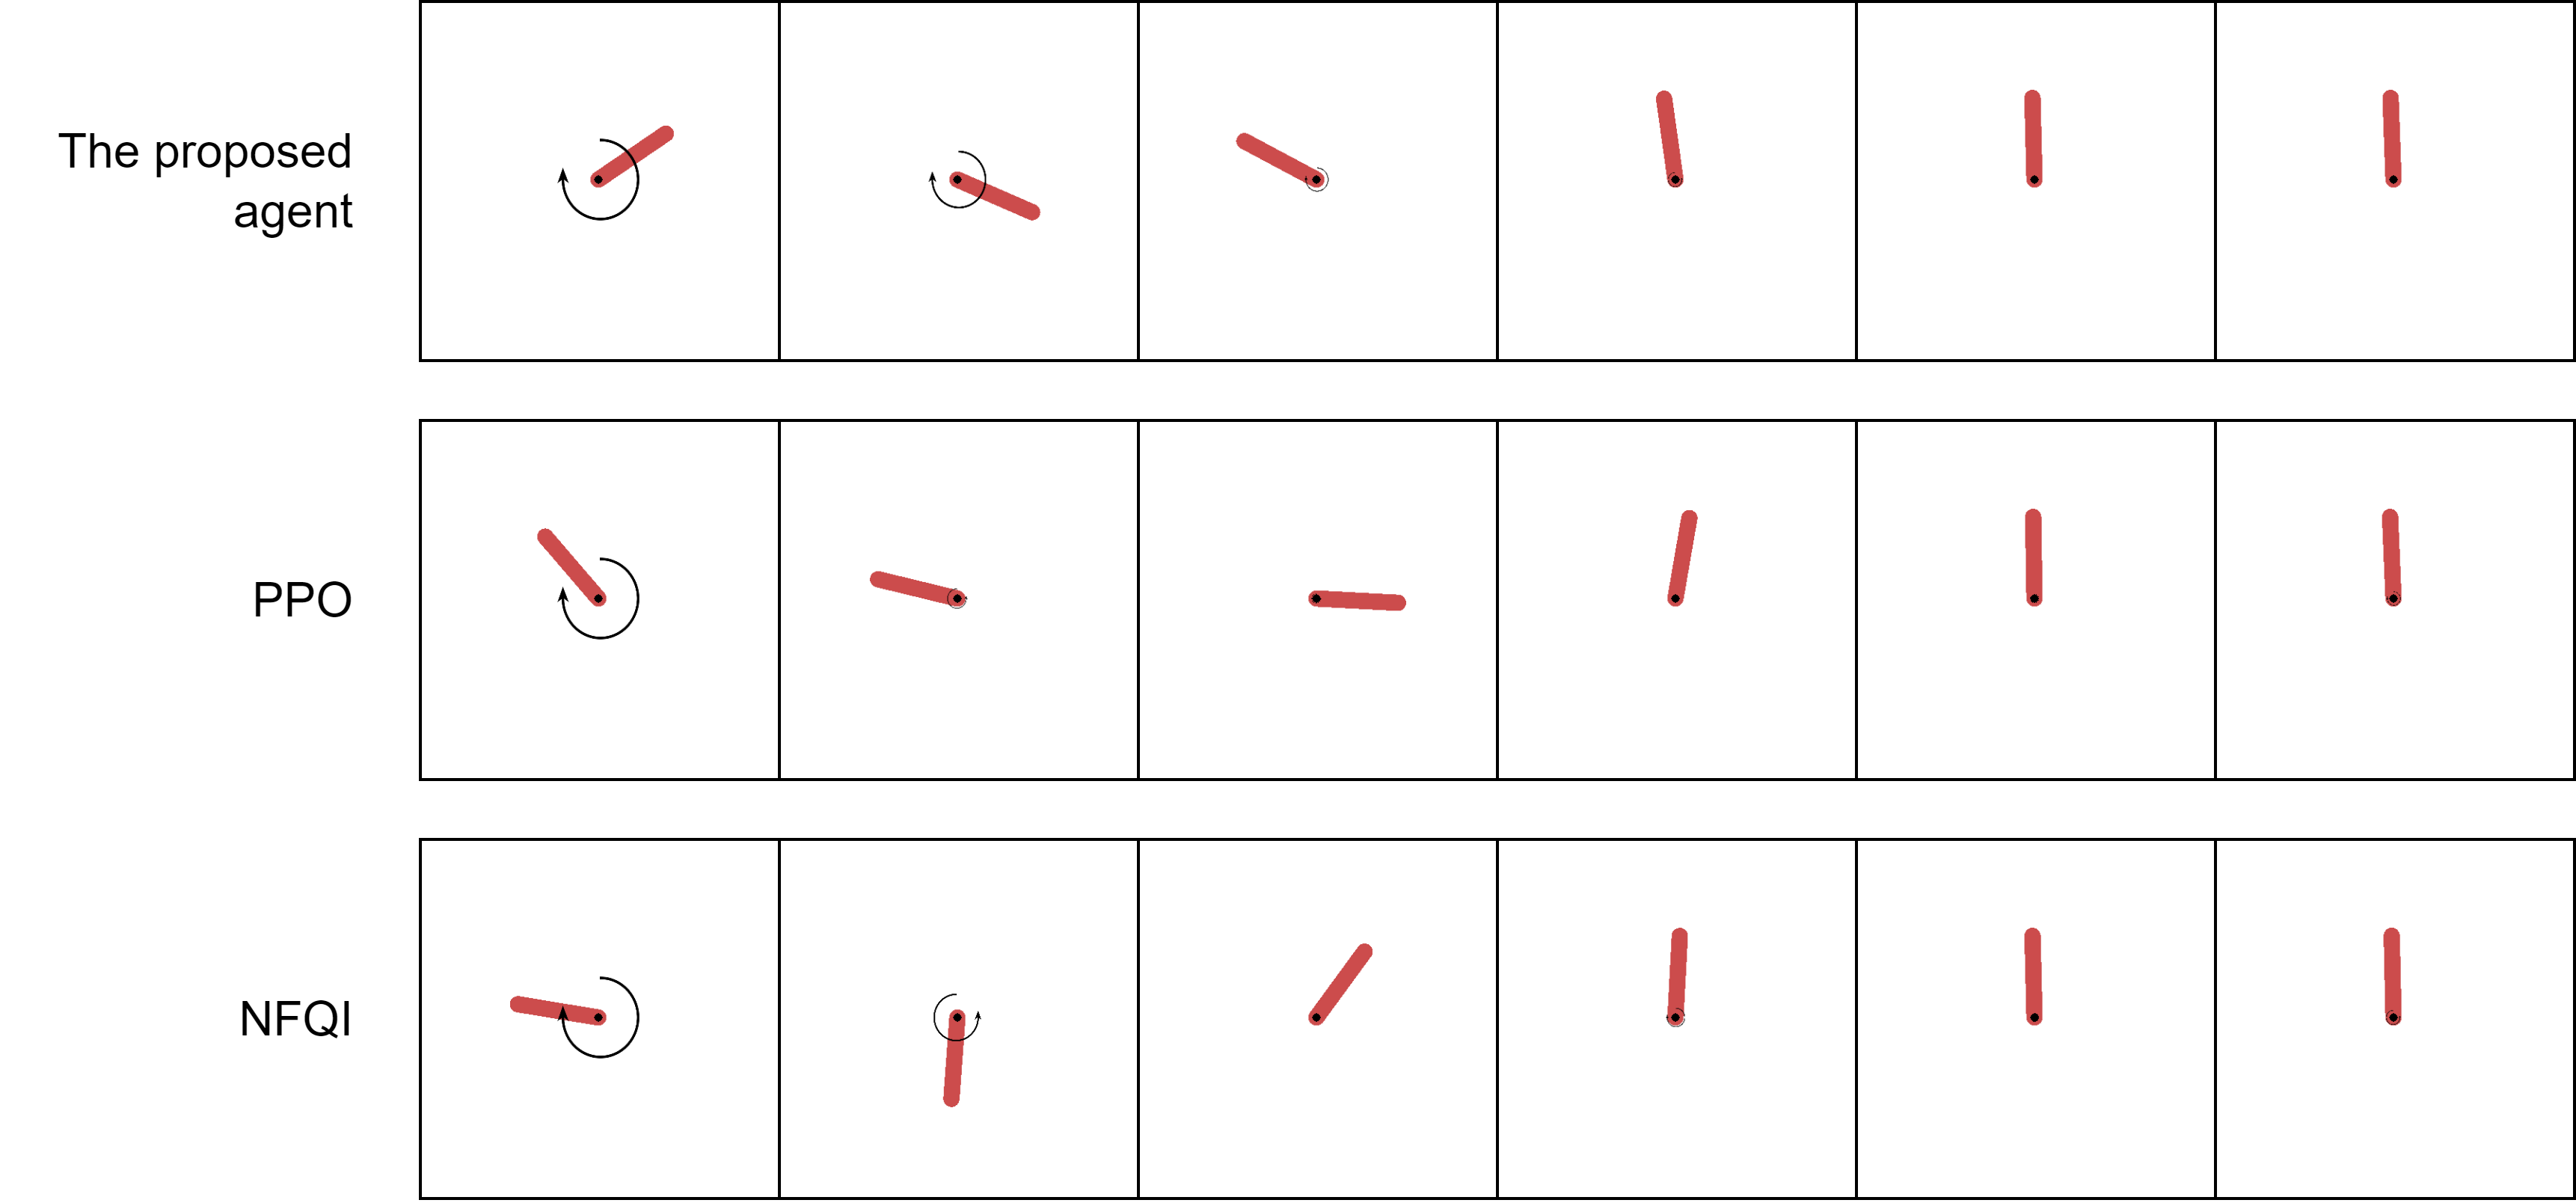
\includegraphics[width=\linewidth]{\FigsDir/Result_Before_Pendulum.png}
      \caption{\centering Pendulum}
    \end{subfigure}
    \caption{\textit{Cont}.}
  \end{figure}
  %
  \begin{figure}[H]\ContinuedFloat
    \centering
    \begin{subfigure}[b]{\linewidth}
      \centering
      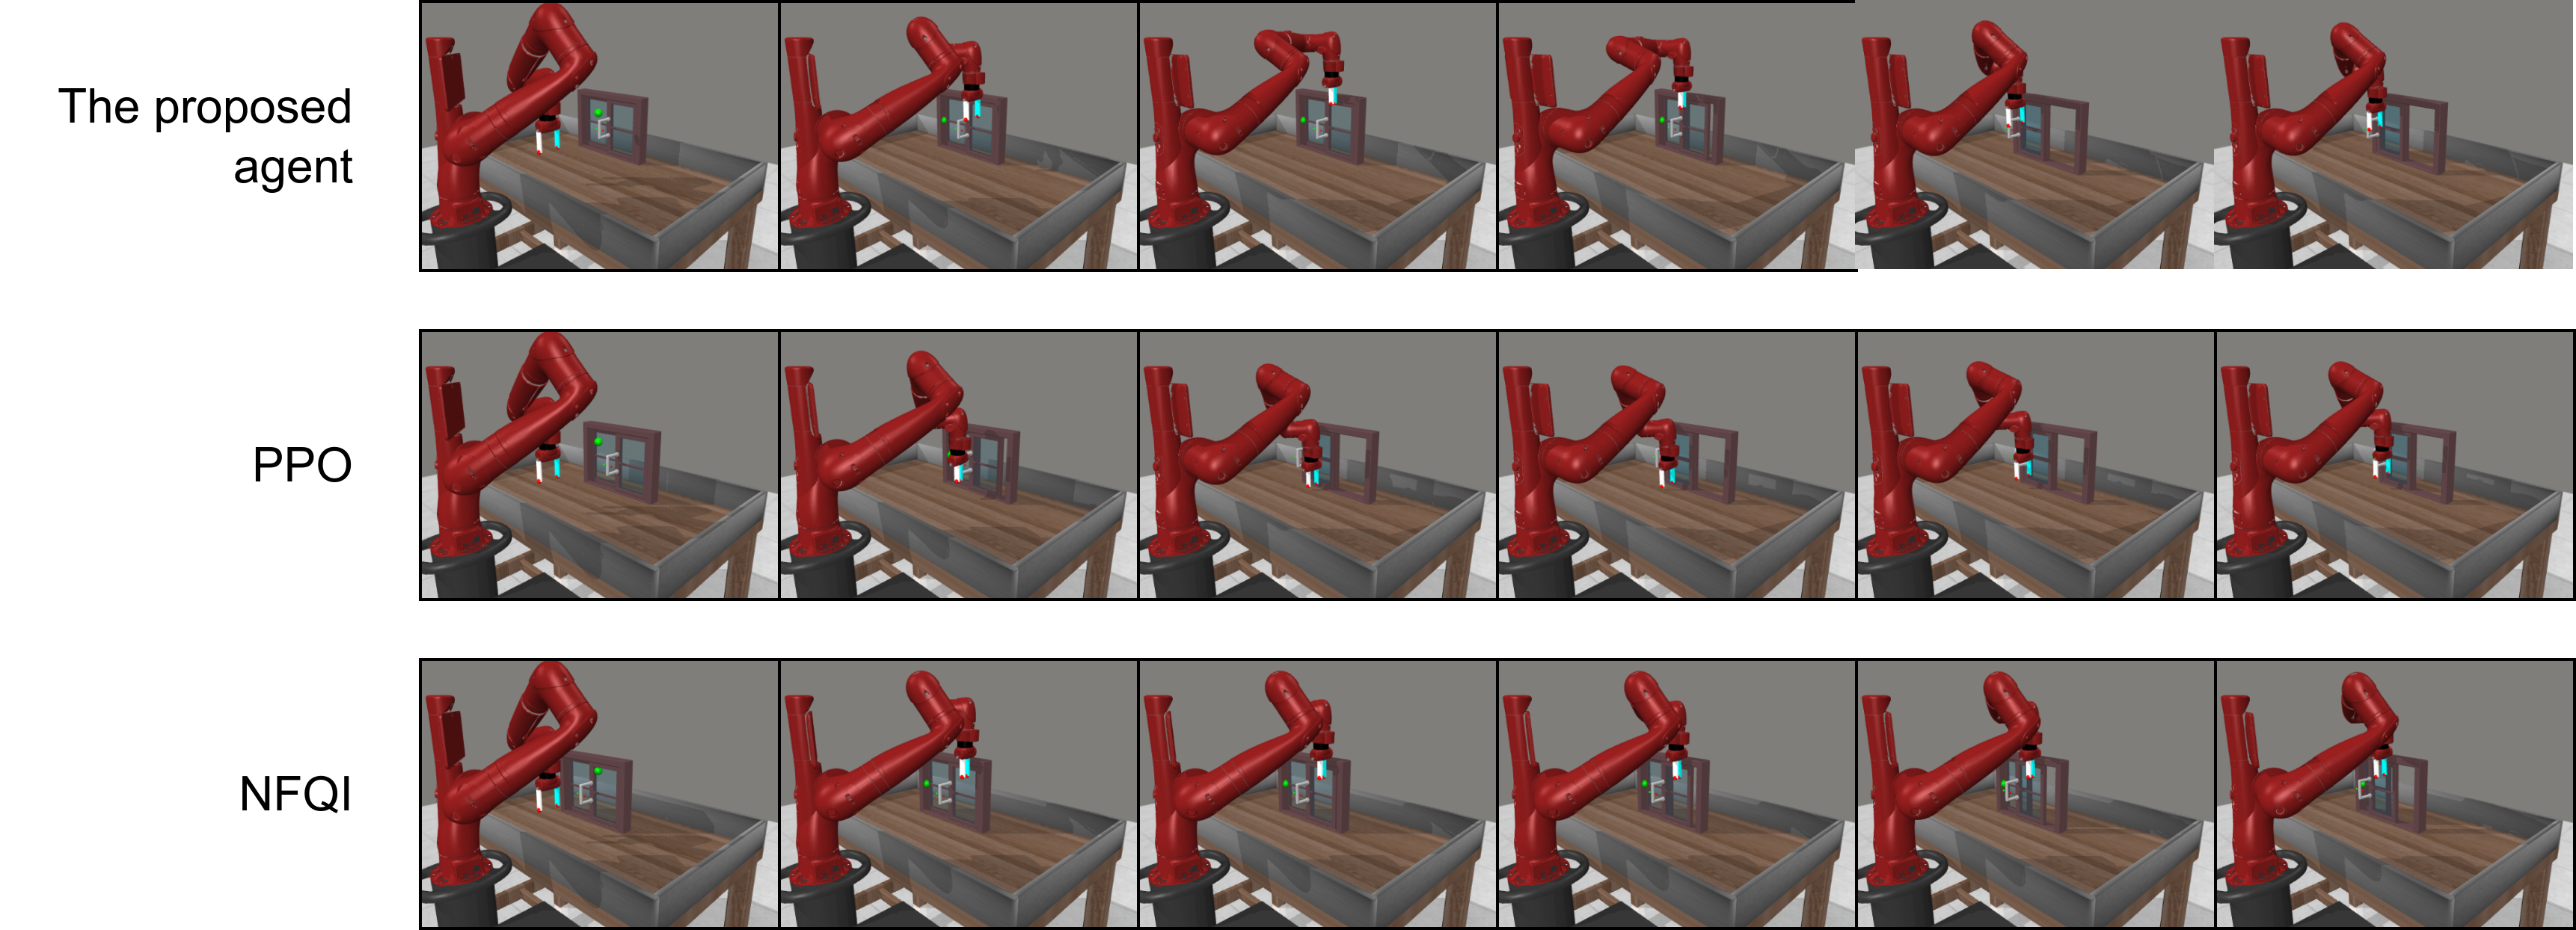
\includegraphics[width=\linewidth]{\FigsDir/Result_Before_WindowOpen.png}
      \caption{\centering WindowOpen}
    \end{subfigure}
    \caption{\textit{Cont}.}
  \end{figure}
  %
  \begin{figure}[H]\ContinuedFloat
    \centering
    \begin{subfigure}[b]{\linewidth}
      \centering
      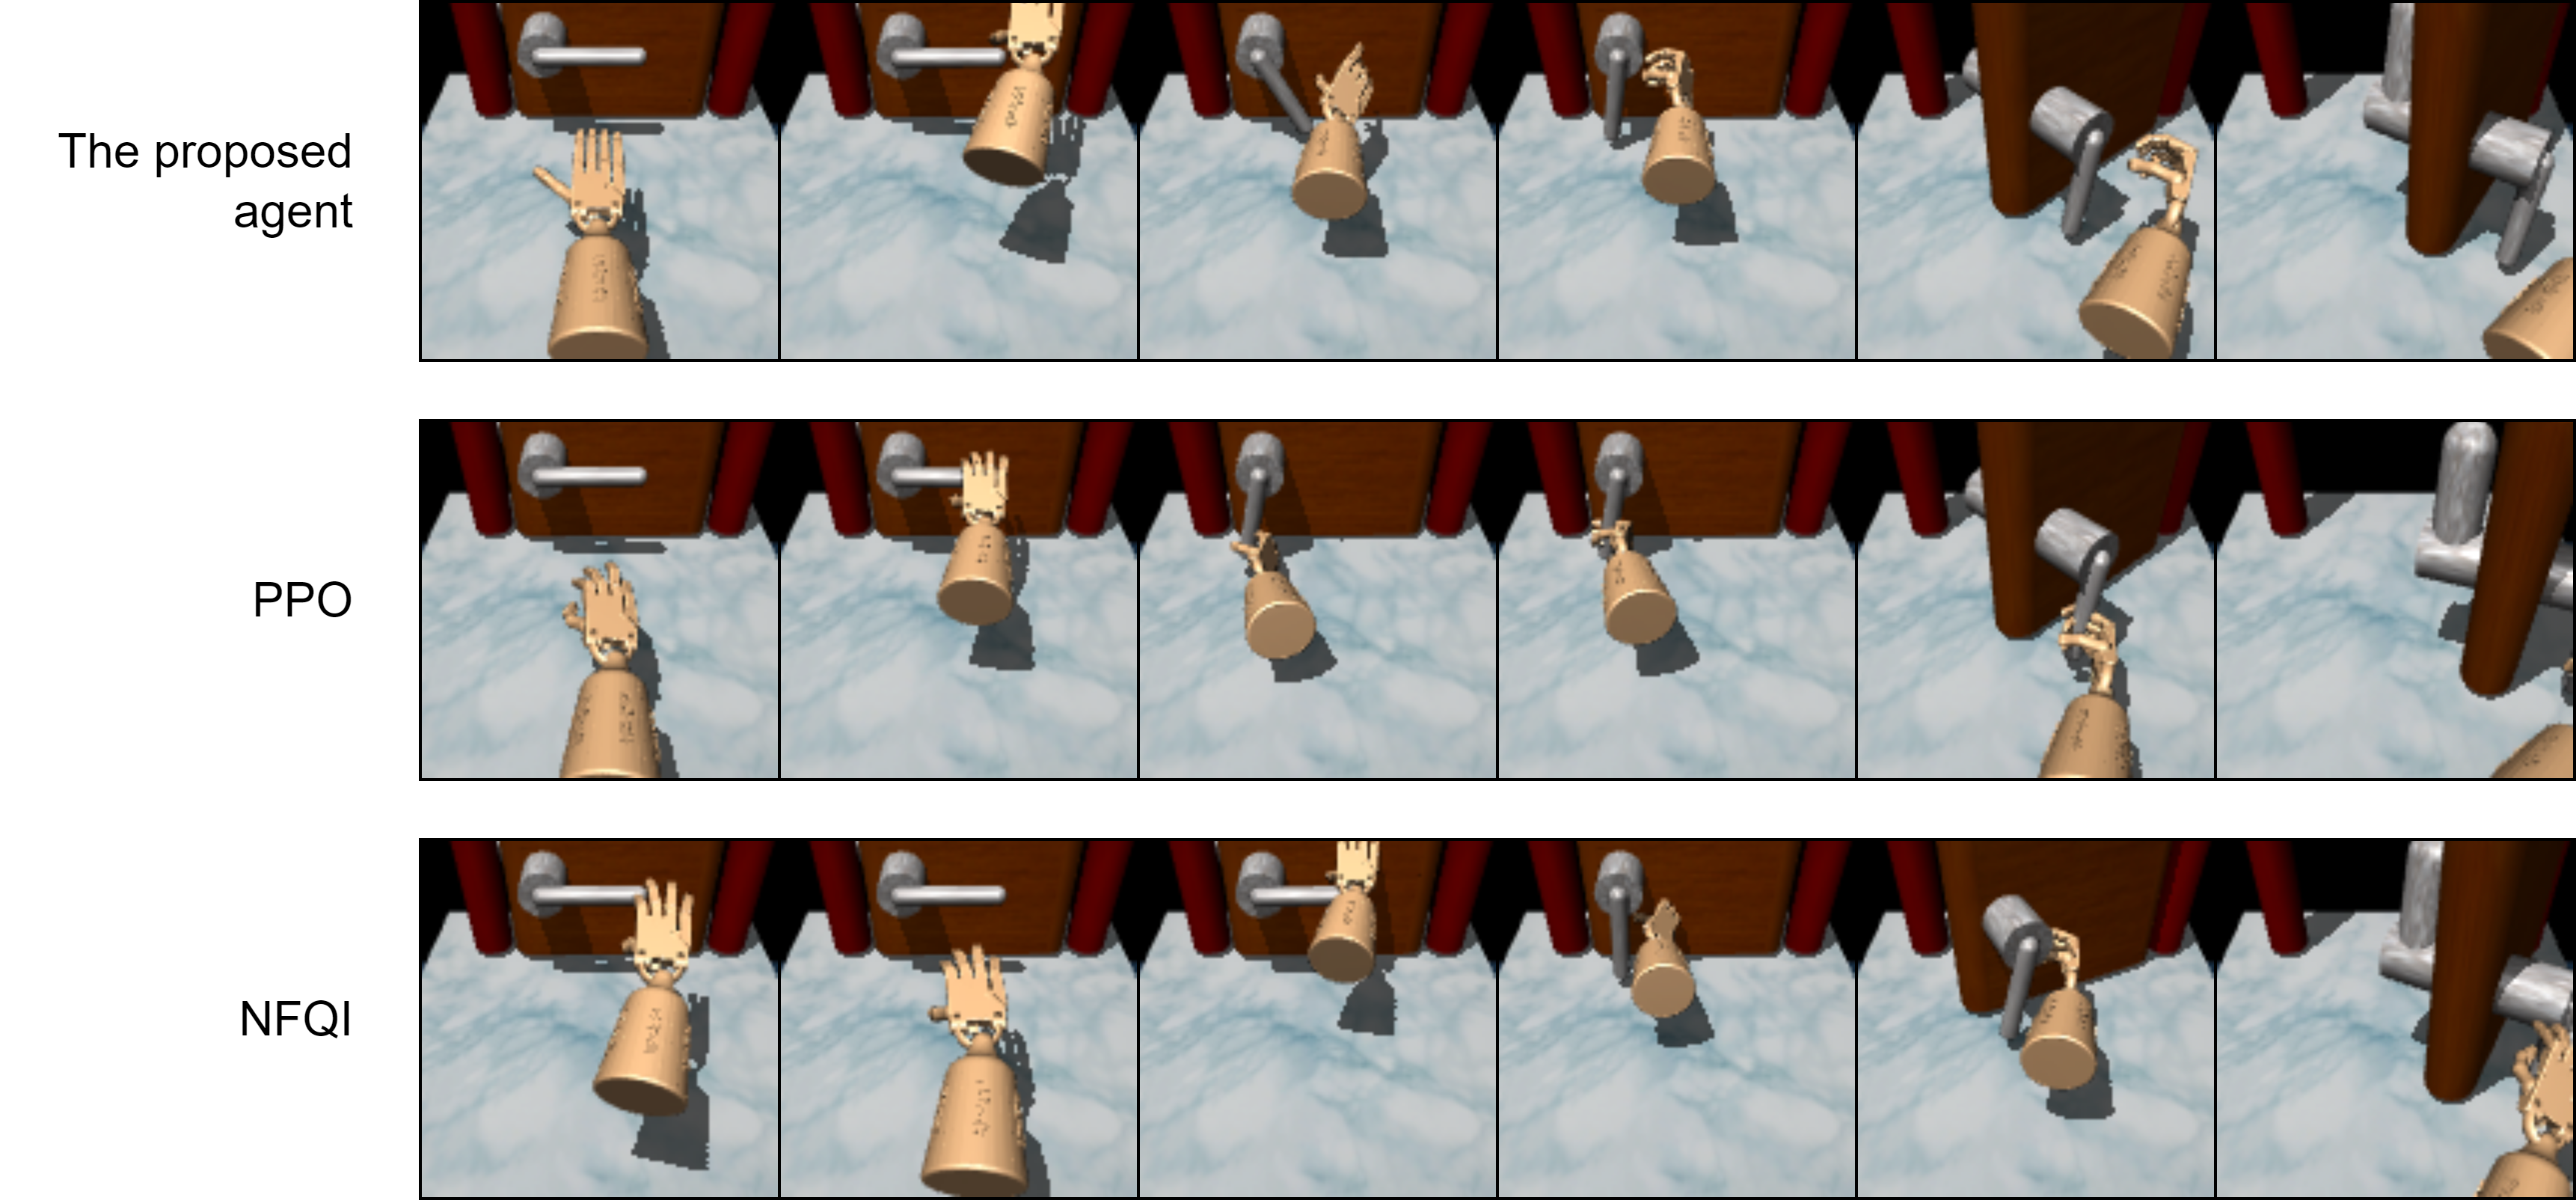
\includegraphics[width=\linewidth]{\FigsDir/Result_Before_Door.png}
      \caption{\centering Door}
    \end{subfigure}
    \caption{A visualization of the behavior of the proposed agent and baselines on source tasks.\label{ch:DTAIL:fig:Result_Before_Source}}
  \end{figure}
\end{landscape}



\subsubsection{Performance of the Proposed Agent on the Target Task after Adaptation}
All agents trained on the source task were adapted to the target task in order to evaluate the performance of the proposed adaptation algorithm in comparison with other transfer learning baselines.
The result is tabulated in Table \ref{ch:DTAIL:tab:Result_SuccessRate_After_Target}.
The behavior of those agents when performing target tasks is visualized in Figure \ref{ch:DTAIL:fig:Result_After_Target}.
It can be seen that the proposed adaptation method and baselines provide comparably similar behaviors in order to solve target tasks.
This result indicated that the proposed method successfully adapted and transferred the agent's knowledge to the new target task.
Moreover, it can be observed from Table \ref{ch:DTAIL:tab:Result_SuccessRate_After_Target} that the proposed method, which is a two-fold method, including the proposed agent and the adaptation algorithm, outperformed other transfer learning-based baselines.
In addition, it performed highly well and consistently on the complex WindowClose and Hammer tasks.
On the other hand,
applying fine tuning to the proposed agent led to a significant reduction in the adapted agent's performance, especially on the complex Hammer task which achieved only a 50\% success rate.
Moreover,
its performance was the lowest compared to other transfer learning baselines.
This indicated that the trained agent on the source task (i.e., Door) failed to transfer its learned knowledge to the target task (i.e., Hammer).
The reason could
be because the adapted agent using fine tuning failed to learn state and action mappings from the source to the target task due to the size of the state and action spaces of those two tasks being different as shown in Table \ref{ch:DTAIL:tab:Tasks}.
This observation indicates that fine tuning was not suitable for the proposed agent.
On the other hand,
applying fine tuning to the PPO agent provided a consistent performance across all three tasks.
At the same time, applying TA-TL to the NFQI agent was not able to produce a high success rate due to the high complexity of the WindowClose and Hammer tasks.


The results demonstrated that the proposed method not only outperformed baselines in terms of success rate on all target tasks, but notably produced a consistently high performance, even on the most difficult task.
This proved the potential of the proposed method in order to tackle the domain and task adaptation problem in imitation learning.
However,
it should be noted that the research objective is not only to achieve high performance on the target task, but also to avoid the performance deterioration on the source task.
Therefore,
the performance of the adapted agent on source tasks will be assessed next in order to evaluate the decline of the agent's performance after adaptation.


\begin{landscape}
  \begin{table}[H]
    \footnotesize
    \caption{The performance of the proposed agent on target tasks after adaptation. \label{ch:DTAIL:tab:Result_SuccessRate_After_Target}}

    \centering
    \setlength{\tabcolsep}{.7mm}{\begin{tabular}{llccc}
        \toprule
         &                                                       & \textbf{CartPole}  & \textbf{WindowClose} & \textbf{Hammer}         \\
        \midrule
        \multirow{4}{*}{Success rate}
         & \DTAIL{}+ \textls[-25]{Proposed adaptation algorithm} & 100\%              & 83\%                 & 82\%                    \\
         & \DTAIL{}+ Fine-tuning                                 & 77\%               & 72\%                 & 50\%                    \\
         & PPO \cite{Baseline_PPO} + Fine-tuning                 & 87\%               & 80\%                 & 77\%                    \\
         & NFQI + TA-TL \cite{Baseline_TATL}                     & 80\%               & 63\%                 & 67\%                    \\
        \midrule
        \multirow{4}{*}{Average cumulative reward}
         & \DTAIL{}+ \textls[-25]{Proposed adaptation algorithm} & $500.00 \pm 0.0$   & $2340.59 \pm 642.69$ & $13,137.42 \pm 2709.57$ \\
         & \DTAIL{}+ Fine-tuning                                 & $433.44 \pm 86.52$ & $1513.07 \pm 566.09$ & $1741.76 \pm 1035.17$   \\
         & PPO \cite{Baseline_PPO} + Fine-tuning                 & $487.63 \pm 32.74$ & $2215.98 \pm 608.33$ & $3022.64 \pm 1115.92$   \\
         & NFQI + TA-TL \cite{Baseline_TATL}                     & $476.63 \pm 61.84$ & $1447.53 \pm 641.16$ & $2591.46 \pm 1231.70$   \\
        \bottomrule
      \end{tabular}}
  \end{table}

  \begin{figure}[H]
    \centering
    %
    \begin{subfigure}[b]{\linewidth}
      \centering
      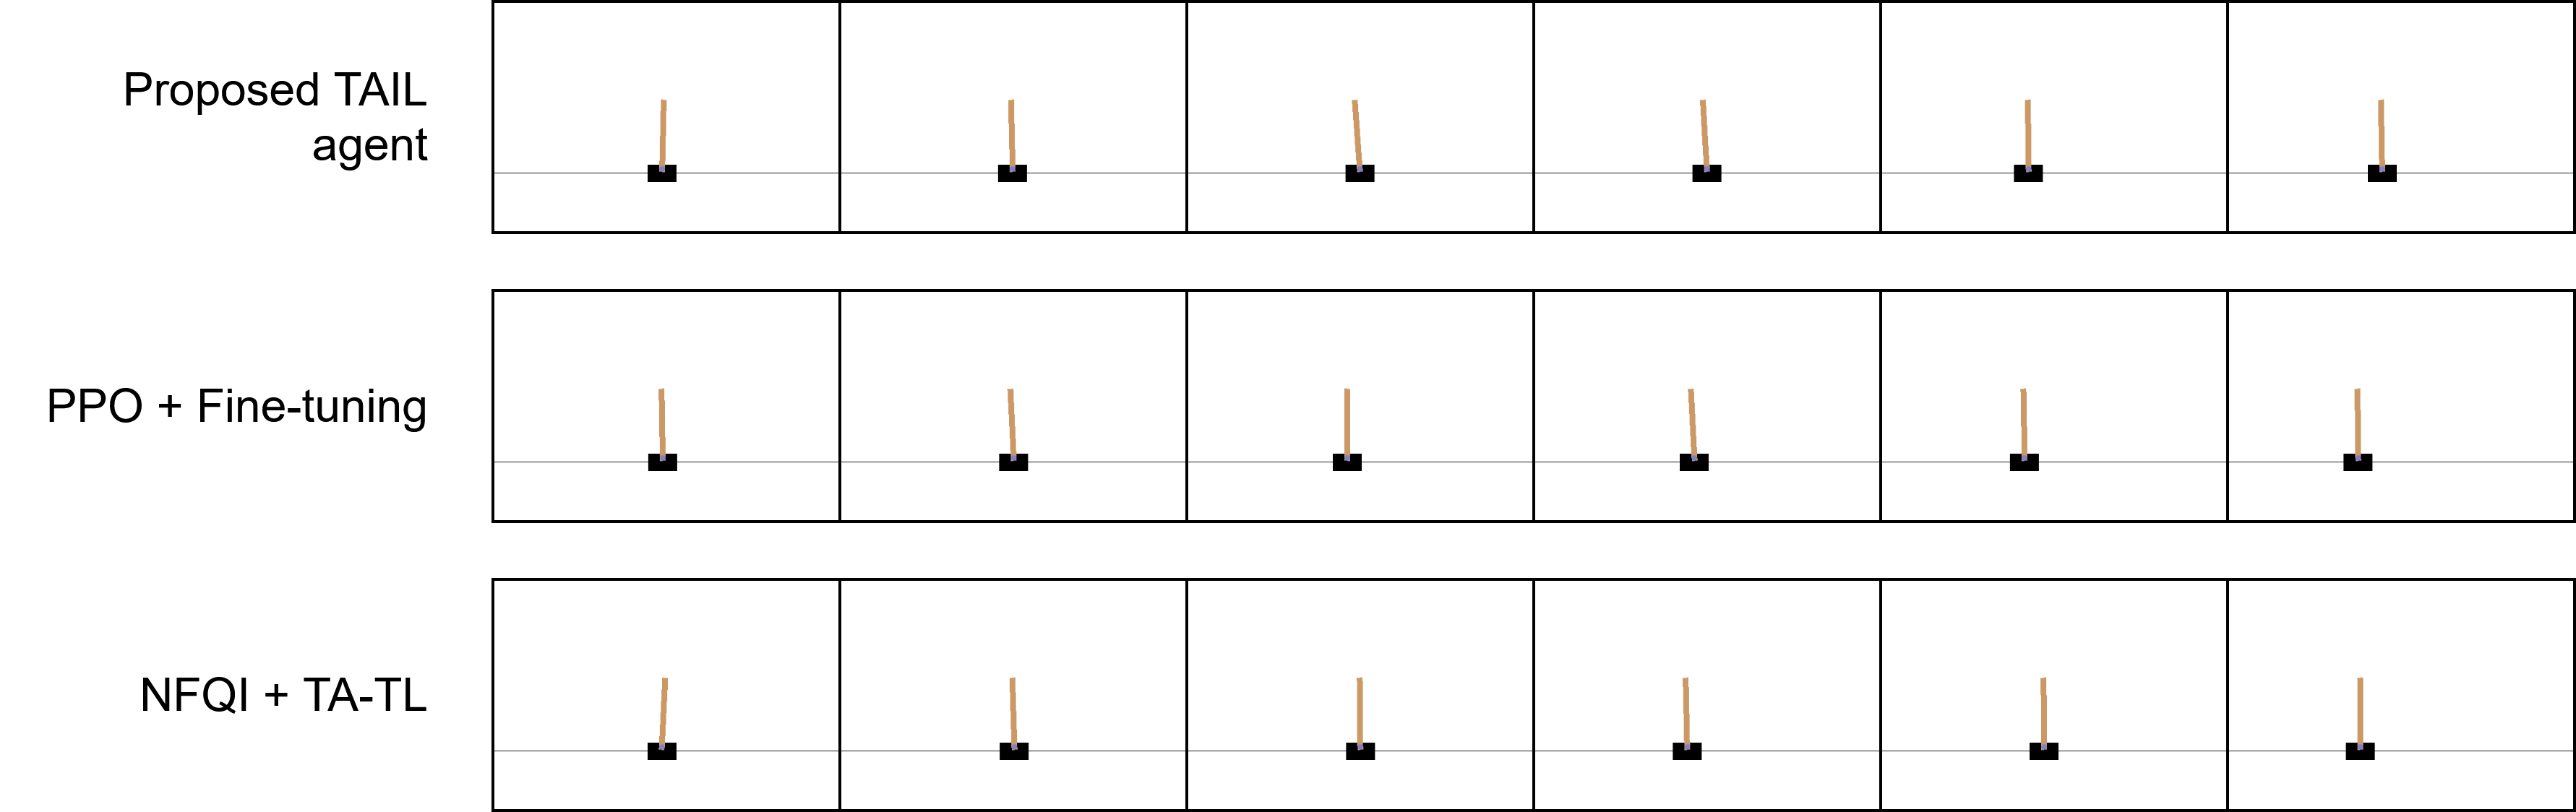
\includegraphics[width=\linewidth]{\FigsDir/Result_After_CartPole.png}
      \caption{\centering CartPole}
    \end{subfigure}
    \caption{\textit{Cont}.}
  \end{figure}
  %
  \begin{figure}[H]\ContinuedFloat
    \begin{subfigure}[b]{\linewidth}
      \centering
      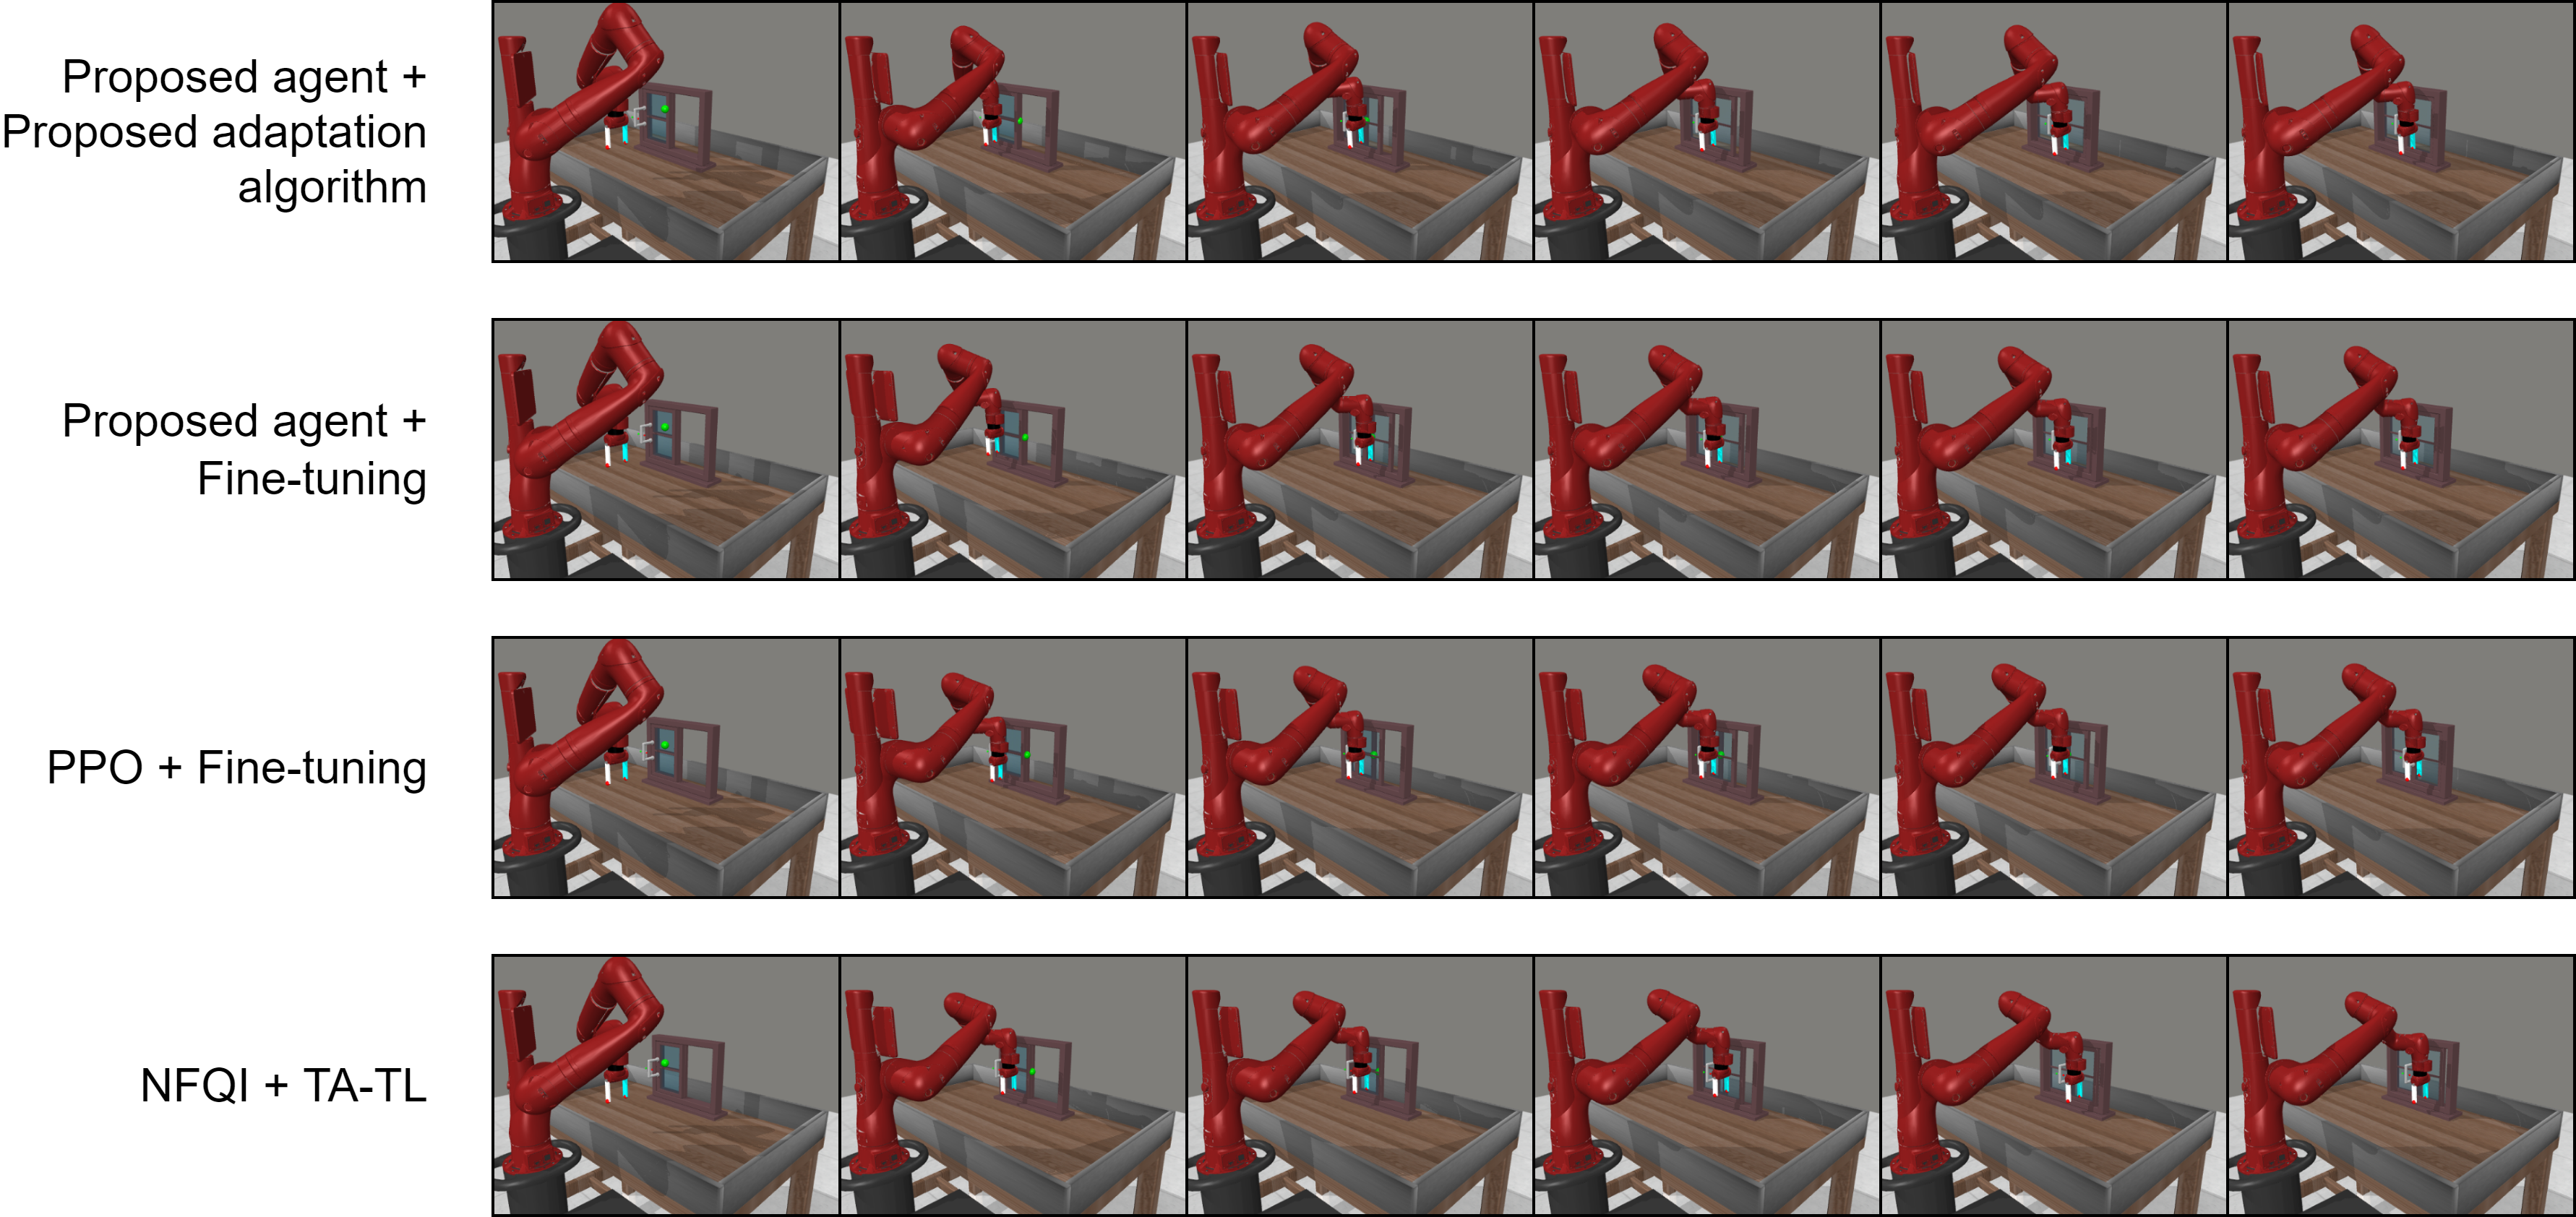
\includegraphics[width=\linewidth]{\FigsDir/Result_After_WindowClose.png}
      \caption{\centering WindowClose}
    \end{subfigure}
    \caption{\textit{Cont}.}
  \end{figure}
  %
  \begin{figure}[H]\ContinuedFloat
    \centering
    %
    \begin{subfigure}[b]{\linewidth}
      \centering
      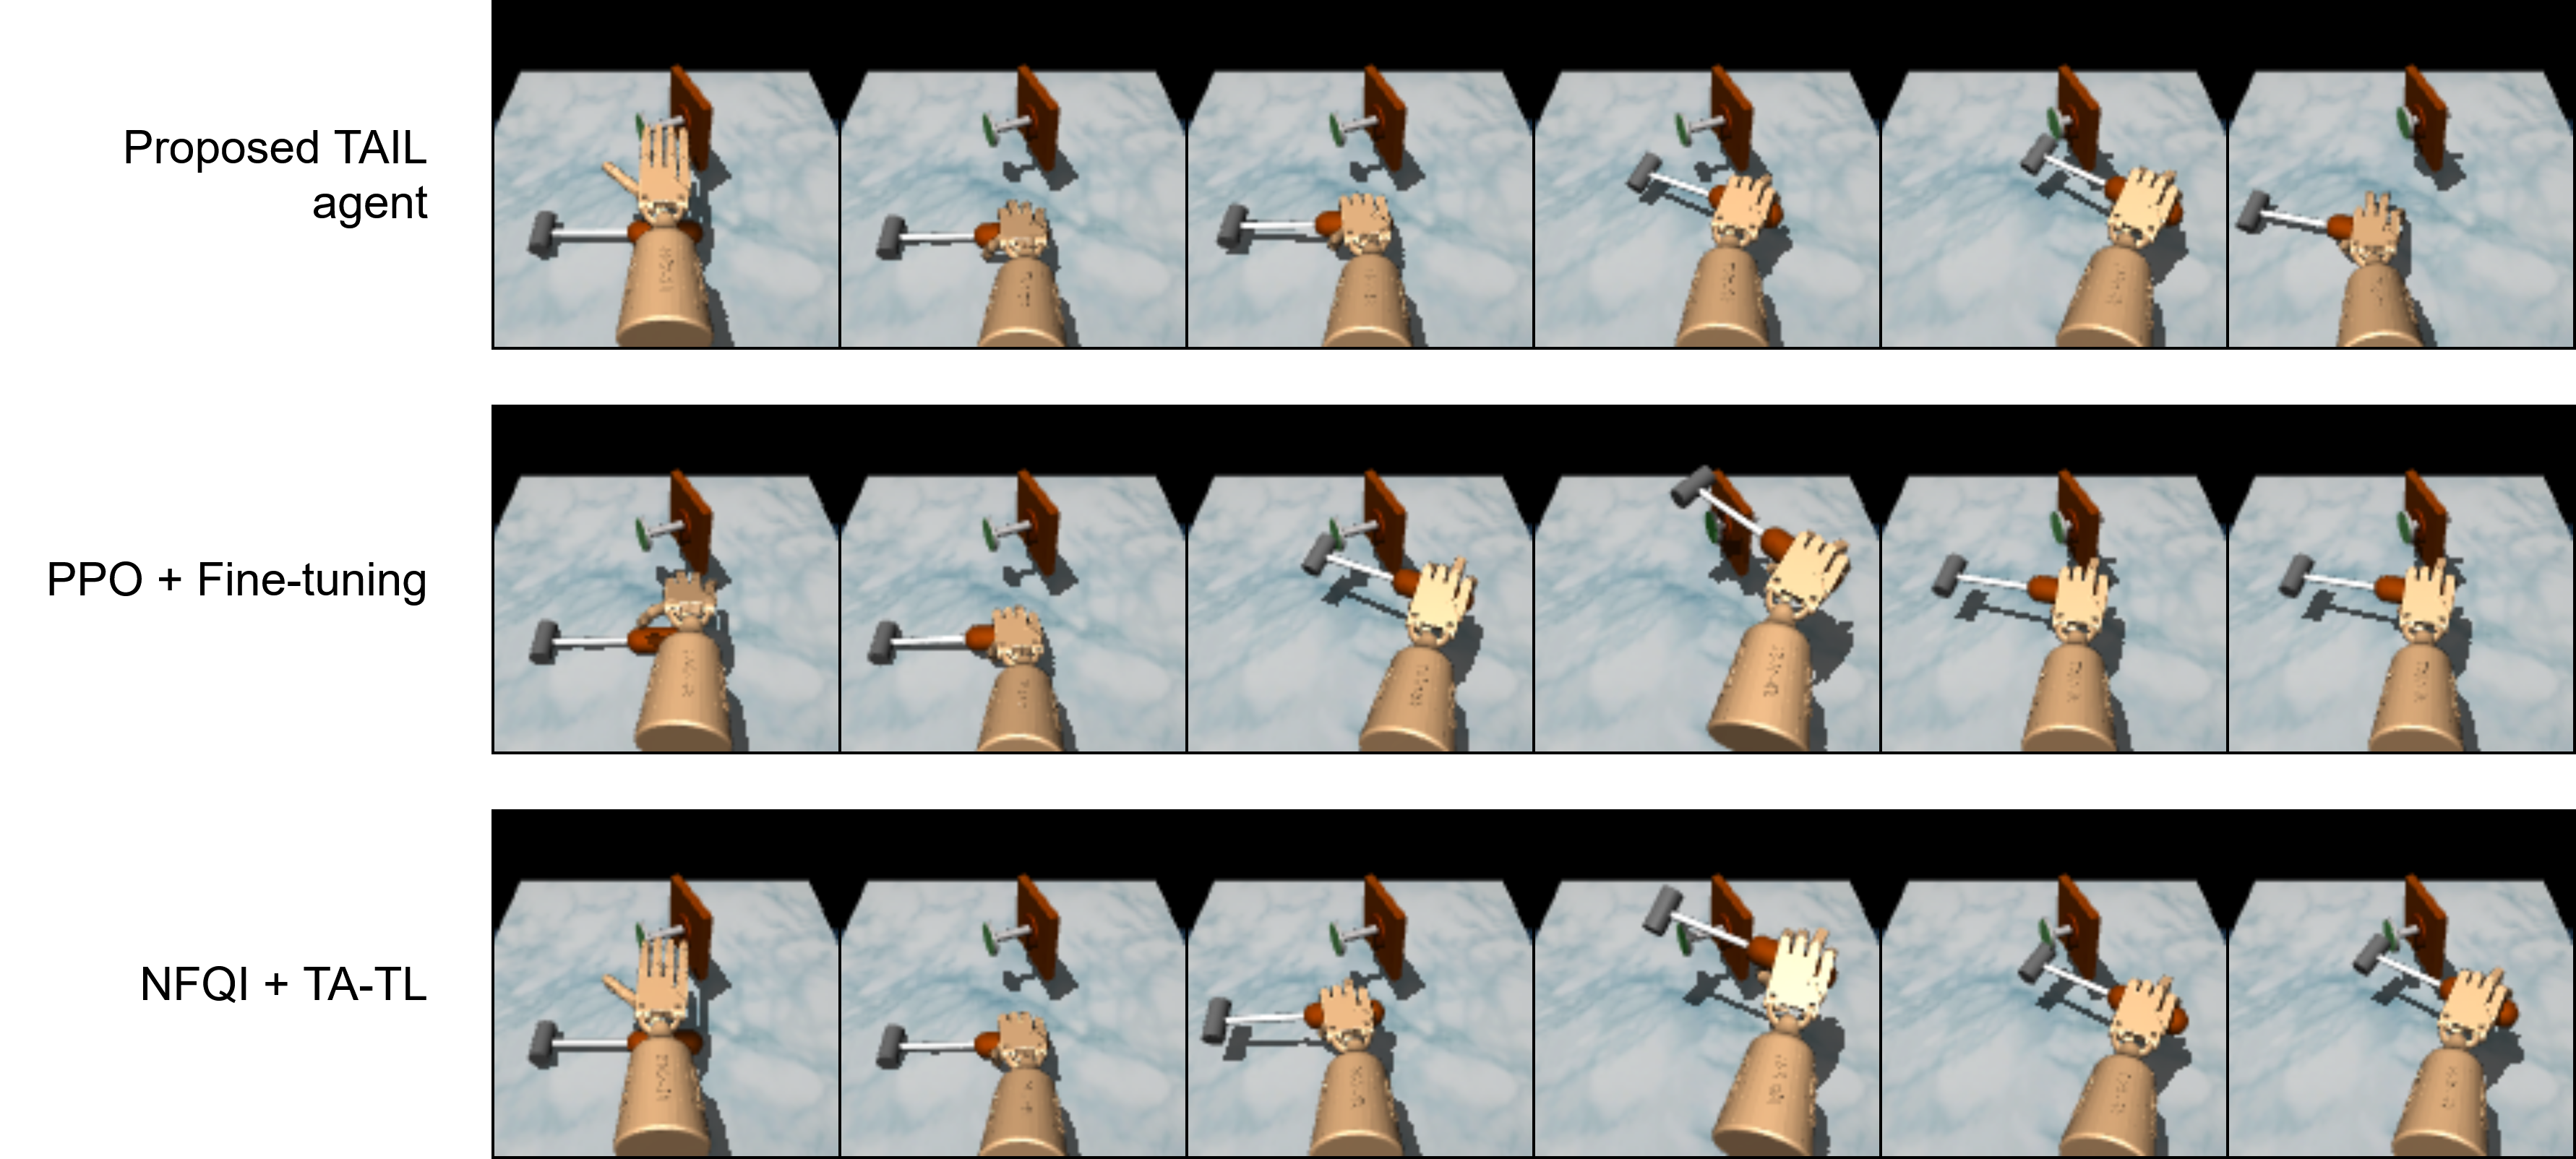
\includegraphics[width=\linewidth]{\FigsDir/Result_After_Hammer.png}
      \caption{\centering Hammer}
    \end{subfigure}
    %
    \caption{A visualization of the behavior of the proposed agent and baselines on target tasks.\label{ch:DTAIL:fig:Result_After_Target}}
  \end{figure}
\end{landscape}
\unskip

\subsubsection{Performance of the Proposed Agent on the Source Task after Adaptation}
Table \ref{ch:DTAIL:tab:Result_SuccessRate_After_Source} shows the deterioration in success rate of the adapted agent on source tasks compared to the one before the adaptation.
The lower value of the deterioration illustrates a better result.
It can be observed that as the difficulty level of the target task increased,
the deterioration became more notable.
In addition,
three baselines were not able to maintain high performance on the source task.
Even on the simple Pendulum task,
the deterioration was extremely high compared to the proposed adaptation algorithm.
This was due to the fact that those transfer learning baselines were designed to optimize the performance of the agent only on the target task.
Thus,
it was obvious that the performance of those adapted agents dropped significantly on the source task.
On the other hand,
the deterioration of the proposed method was the lowest compared to other baselines,
which indicated that the proposed adaptation algorithm successfully retained the learned knowledge from the source tasks and reduced the negative effect of catastrophic forgetting.

\begin{landscape}
  \begin{table}[H]
    \caption{The performance of the proposed agent on source tasks after adaptation. These scores represent the deterioration in success rate compared to the one before the adaptation. \label{ch:DTAIL:tab:Result_SuccessRate_After_Source}}

    \centering
    \begin{tabular}{lcccc}
      \toprule
                                              & \textbf{Pendulum} & \textbf{WindowOpen} & \textbf{Door} \\
      \midrule
      \DTAIL{}+ Proposed adaptation algorithm & 18\%              & 32\%                & 44\%          \\
      \DTAIL{}+ Fine-Tuning                   & 41\%              & 73\%                & 74\%          \\
      PPO \cite{Baseline_PPO} + Fine-tuning   & 32\%              & 58\%                & 83\%          \\
      NFQI + TA-TL \cite{Baseline_TATL}       & 24\%              & 62\%                & 51\%          \\
      \bottomrule
    \end{tabular}
  \end{table}
\end{landscape}

\subsubsection{Computational Complexity}
Besides evaluating the performance of the proposed task adaptation method in terms of success rate,
its computational cost was also assessed in order to provide an adequate study of its overall performance.
Table \ref{ch:DTAIL:tab:Result_Cost} shows the training time required to adapt a trained agent to a new target task in each experiment.
It can be observed that the training time of the proposed adaptation method was slightly better than the training time when applying fine tuning to PPO, especially on two complex WindowOpen-WindowClose and Door--Hammer experiments.
On the other hand, compared to TA-TL, the proposed adaptation method required a higher training time on all three experiments.
This result was expected since,
during the proposed adaptation process,
the agent had to not only learn the new task, but also review the previously learned source task.
However,
it should be noted that the training time of the proposed adaptation method can be further improved by leveraging the parallel training process \cite{DL_Lib_StableBaselines3, DL_Lib_Tianshou}.

\begin{landscape}
  \begin{table}[H]
    \caption{The training time (s/epoch) of the proposed task adaptation algorithm.\label{ch:DTAIL:tab:Result_Cost}}

    \centering
    \begin{tabular}{p{5.5cm}ccc}
      \toprule
                                              & \textbf{Pendulum--CartPole} & \textbf{WindowOpen--WindowClose} & \textbf{Door--Hammer} \\
      \midrule
      \DTAIL{}+ Proposed adaptation algorithm & 87.051                      & 163.768                          & 503.19                \\
      \DTAIL{}+ Fine-tuning                   & 74.680                      & 114.290                          & 321.87                \\
      PPO \cite{Baseline_PPO} + Fine-tuning   & 86.801                      & 184.472                          & 557.416               \\
      NFQI + TA-TL \cite{Baseline_TATL}       & 58.499                      & 121.510                          & 352.53                \\
      \bottomrule
    \end{tabular}
  \end{table}
\end{landscape}
